% Options for packages loaded elsewhere
\PassOptionsToPackage{unicode}{hyperref}
\PassOptionsToPackage{hyphens}{url}
%
\documentclass[
]{book}
\usepackage{amsmath,amssymb}
\usepackage{lmodern}
\usepackage{ifxetex,ifluatex}
\ifnum 0\ifxetex 1\fi\ifluatex 1\fi=0 % if pdftex
  \usepackage[T1]{fontenc}
  \usepackage[utf8]{inputenc}
  \usepackage{textcomp} % provide euro and other symbols
\else % if luatex or xetex
  \usepackage{unicode-math}
  \defaultfontfeatures{Scale=MatchLowercase}
  \defaultfontfeatures[\rmfamily]{Ligatures=TeX,Scale=1}
\fi
% Use upquote if available, for straight quotes in verbatim environments
\IfFileExists{upquote.sty}{\usepackage{upquote}}{}
\IfFileExists{microtype.sty}{% use microtype if available
  \usepackage[]{microtype}
  \UseMicrotypeSet[protrusion]{basicmath} % disable protrusion for tt fonts
}{}
\makeatletter
\@ifundefined{KOMAClassName}{% if non-KOMA class
  \IfFileExists{parskip.sty}{%
    \usepackage{parskip}
  }{% else
    \setlength{\parindent}{0pt}
    \setlength{\parskip}{6pt plus 2pt minus 1pt}}
}{% if KOMA class
  \KOMAoptions{parskip=half}}
\makeatother
\usepackage{xcolor}
\IfFileExists{xurl.sty}{\usepackage{xurl}}{} % add URL line breaks if available
\IfFileExists{bookmark.sty}{\usepackage{bookmark}}{\usepackage{hyperref}}
\hypersetup{
  pdftitle={A New PPB Toolkit},
  pdfauthor={Sergio Castro and Matteo Petitti},
  hidelinks,
  pdfcreator={LaTeX via pandoc}}
\urlstyle{same} % disable monospaced font for URLs
\usepackage{color}
\usepackage{fancyvrb}
\newcommand{\VerbBar}{|}
\newcommand{\VERB}{\Verb[commandchars=\\\{\}]}
\DefineVerbatimEnvironment{Highlighting}{Verbatim}{commandchars=\\\{\}}
% Add ',fontsize=\small' for more characters per line
\usepackage{framed}
\definecolor{shadecolor}{RGB}{248,248,248}
\newenvironment{Shaded}{\begin{snugshade}}{\end{snugshade}}
\newcommand{\AlertTok}[1]{\textcolor[rgb]{0.94,0.16,0.16}{#1}}
\newcommand{\AnnotationTok}[1]{\textcolor[rgb]{0.56,0.35,0.01}{\textbf{\textit{#1}}}}
\newcommand{\AttributeTok}[1]{\textcolor[rgb]{0.77,0.63,0.00}{#1}}
\newcommand{\BaseNTok}[1]{\textcolor[rgb]{0.00,0.00,0.81}{#1}}
\newcommand{\BuiltInTok}[1]{#1}
\newcommand{\CharTok}[1]{\textcolor[rgb]{0.31,0.60,0.02}{#1}}
\newcommand{\CommentTok}[1]{\textcolor[rgb]{0.56,0.35,0.01}{\textit{#1}}}
\newcommand{\CommentVarTok}[1]{\textcolor[rgb]{0.56,0.35,0.01}{\textbf{\textit{#1}}}}
\newcommand{\ConstantTok}[1]{\textcolor[rgb]{0.00,0.00,0.00}{#1}}
\newcommand{\ControlFlowTok}[1]{\textcolor[rgb]{0.13,0.29,0.53}{\textbf{#1}}}
\newcommand{\DataTypeTok}[1]{\textcolor[rgb]{0.13,0.29,0.53}{#1}}
\newcommand{\DecValTok}[1]{\textcolor[rgb]{0.00,0.00,0.81}{#1}}
\newcommand{\DocumentationTok}[1]{\textcolor[rgb]{0.56,0.35,0.01}{\textbf{\textit{#1}}}}
\newcommand{\ErrorTok}[1]{\textcolor[rgb]{0.64,0.00,0.00}{\textbf{#1}}}
\newcommand{\ExtensionTok}[1]{#1}
\newcommand{\FloatTok}[1]{\textcolor[rgb]{0.00,0.00,0.81}{#1}}
\newcommand{\FunctionTok}[1]{\textcolor[rgb]{0.00,0.00,0.00}{#1}}
\newcommand{\ImportTok}[1]{#1}
\newcommand{\InformationTok}[1]{\textcolor[rgb]{0.56,0.35,0.01}{\textbf{\textit{#1}}}}
\newcommand{\KeywordTok}[1]{\textcolor[rgb]{0.13,0.29,0.53}{\textbf{#1}}}
\newcommand{\NormalTok}[1]{#1}
\newcommand{\OperatorTok}[1]{\textcolor[rgb]{0.81,0.36,0.00}{\textbf{#1}}}
\newcommand{\OtherTok}[1]{\textcolor[rgb]{0.56,0.35,0.01}{#1}}
\newcommand{\PreprocessorTok}[1]{\textcolor[rgb]{0.56,0.35,0.01}{\textit{#1}}}
\newcommand{\RegionMarkerTok}[1]{#1}
\newcommand{\SpecialCharTok}[1]{\textcolor[rgb]{0.00,0.00,0.00}{#1}}
\newcommand{\SpecialStringTok}[1]{\textcolor[rgb]{0.31,0.60,0.02}{#1}}
\newcommand{\StringTok}[1]{\textcolor[rgb]{0.31,0.60,0.02}{#1}}
\newcommand{\VariableTok}[1]{\textcolor[rgb]{0.00,0.00,0.00}{#1}}
\newcommand{\VerbatimStringTok}[1]{\textcolor[rgb]{0.31,0.60,0.02}{#1}}
\newcommand{\WarningTok}[1]{\textcolor[rgb]{0.56,0.35,0.01}{\textbf{\textit{#1}}}}
\usepackage{longtable,booktabs,array}
\usepackage{calc} % for calculating minipage widths
% Correct order of tables after \paragraph or \subparagraph
\usepackage{etoolbox}
\makeatletter
\patchcmd\longtable{\par}{\if@noskipsec\mbox{}\fi\par}{}{}
\makeatother
% Allow footnotes in longtable head/foot
\IfFileExists{footnotehyper.sty}{\usepackage{footnotehyper}}{\usepackage{footnote}}
\makesavenoteenv{longtable}
\usepackage{graphicx}
\makeatletter
\def\maxwidth{\ifdim\Gin@nat@width>\linewidth\linewidth\else\Gin@nat@width\fi}
\def\maxheight{\ifdim\Gin@nat@height>\textheight\textheight\else\Gin@nat@height\fi}
\makeatother
% Scale images if necessary, so that they will not overflow the page
% margins by default, and it is still possible to overwrite the defaults
% using explicit options in \includegraphics[width, height, ...]{}
\setkeys{Gin}{width=\maxwidth,height=\maxheight,keepaspectratio}
% Set default figure placement to htbp
\makeatletter
\def\fps@figure{htbp}
\makeatother
\setlength{\emergencystretch}{3em} % prevent overfull lines
\providecommand{\tightlist}{%
  \setlength{\itemsep}{0pt}\setlength{\parskip}{0pt}}
\setcounter{secnumdepth}{5}
\usepackage{booktabs}
\ifluatex
  \usepackage{selnolig}  % disable illegal ligatures
\fi
\usepackage[]{natbib}
\bibliographystyle{apalike}

\title{A New PPB Toolkit}
\author{Sergio Castro and Matteo Petitti}
\date{2021-06-04}

\begin{document}
\maketitle

{
\setcounter{tocdepth}{1}
\tableofcontents
}
\hypertarget{foreword}{%
\chapter{Foreword}\label{foreword}}

This is a very important foreword.
.

\hypertarget{intro}{%
\chapter{Introduction}\label{intro}}

\#A beautiful introduction goes here.

\hypertarget{first-steps-in-r}{%
\chapter{First steps in R}\label{first-steps-in-r}}

If you already know the basics of R, you can skip this section!

\hypertarget{why-r}{%
\section{Why R?}\label{why-r}}

\begin{itemize}
\item
  Open Source.\\
  Constantly uptaed by users around the world.
\item
  Polifunctional.\\
  Data Management, Statistica Analysis and Data Visualization.
\item
  Reproducibile.\\
  You can share your methods and results.
\end{itemize}

\hypertarget{lets-start}{%
\section{Let's start}\label{lets-start}}

Rstudio is like a calculator (but very powerful)
Try to write on the console, and then click the Enter button.:

\begin{Shaded}
\begin{Highlighting}[]
\DecValTok{1}\SpecialCharTok{+}\DecValTok{1} 
\end{Highlighting}
\end{Shaded}

\begin{verbatim}
## [1] 2
\end{verbatim}

Try to do the same on the text editor (and then type Ctrl+Enter)

\begin{Shaded}
\begin{Highlighting}[]
\DecValTok{1}\SpecialCharTok{+}\DecValTok{1}
\end{Highlighting}
\end{Shaded}

\begin{verbatim}
## [1] 2
\end{verbatim}

\hypertarget{other-arithmetic-functions.}{%
\section{Other Arithmetic functions.}\label{other-arithmetic-functions.}}

6x9

\begin{Shaded}
\begin{Highlighting}[]
\DecValTok{6}\SpecialCharTok{*}\DecValTok{9}
\end{Highlighting}
\end{Shaded}

\begin{verbatim}
## [1] 54
\end{verbatim}

3/2

\begin{Shaded}
\begin{Highlighting}[]
\DecValTok{3}\SpecialCharTok{/}\DecValTok{2}
\end{Highlighting}
\end{Shaded}

\begin{verbatim}
## [1] 1.5
\end{verbatim}

10+20/(2)

\begin{Shaded}
\begin{Highlighting}[]
\NormalTok{(}\DecValTok{10}\SpecialCharTok{+}\DecValTok{20}\NormalTok{)}\SpecialCharTok{/}\DecValTok{2}
\end{Highlighting}
\end{Shaded}

\begin{verbatim}
## [1] 15
\end{verbatim}

Square root of 2

\begin{Shaded}
\begin{Highlighting}[]
\FunctionTok{sqrt}\NormalTok{(}\DecValTok{2}\NormalTok{)}
\end{Highlighting}
\end{Shaded}

\begin{verbatim}
## [1] 1.414214
\end{verbatim}

10 power of 2

\begin{Shaded}
\begin{Highlighting}[]
\DecValTok{10}\SpecialCharTok{\^{}}\DecValTok{2}
\end{Highlighting}
\end{Shaded}

\begin{verbatim}
## [1] 100
\end{verbatim}

Logarithm of 10

\begin{Shaded}
\begin{Highlighting}[]
\FunctionTok{log}\NormalTok{(}\DecValTok{10}\NormalTok{)}
\end{Highlighting}
\end{Shaded}

\begin{verbatim}
## [1] 2.302585
\end{verbatim}

\hypertarget{functions}{%
\section{Functions}\label{functions}}

Functions are the base of, they are always written followed by a parenthesis.
What is between parenthesis is called ``arguments''.

Three examples:

\begin{verbatim}
 Mean = mean()
 Standard deviation =  sd()
 Concatenate =  c()   
 
\end{verbatim}

How to use them?

\begin{Shaded}
\begin{Highlighting}[]
\CommentTok{\#Put together four elements.}
\FunctionTok{c}\NormalTok{(}\DecValTok{1}\NormalTok{,}\DecValTok{2}\NormalTok{,}\DecValTok{3}\NormalTok{,}\DecValTok{4}\NormalTok{)}
\end{Highlighting}
\end{Shaded}

\begin{verbatim}
## [1] 1 2 3 4
\end{verbatim}

\begin{Shaded}
\begin{Highlighting}[]
\CommentTok{\#Estimate the mean of these four elements.}
\FunctionTok{mean}\NormalTok{(}\FunctionTok{c}\NormalTok{(}\DecValTok{1}\NormalTok{,}\DecValTok{2}\NormalTok{,}\DecValTok{3}\NormalTok{,}\DecValTok{4}\NormalTok{))}
\end{Highlighting}
\end{Shaded}

\begin{verbatim}
## [1] 2.5
\end{verbatim}

\begin{Shaded}
\begin{Highlighting}[]
\CommentTok{\#Estimate the Standard Deviation of these four elements.}
\FunctionTok{sd}\NormalTok{ (}\FunctionTok{c}\NormalTok{(}\DecValTok{1}\NormalTok{,}\DecValTok{2}\NormalTok{,}\DecValTok{3}\NormalTok{,}\DecValTok{4}\NormalTok{))}
\end{Highlighting}
\end{Shaded}

\begin{verbatim}
## [1] 1.290994
\end{verbatim}

\hypertarget{objects}{%
\section{Objects}\label{objects}}

Mostly everything in R are ``Objects''. They can be numbers, characters, databases and other things.

You can see your objects in the upper right window of RStudio, called environment.

You can create objects by using ` = ' o ` \textless- `

Example:

\begin{Shaded}
\begin{Highlighting}[]
\CommentTok{\#Create an object called x}
\NormalTok{x }\OtherTok{=} \FunctionTok{c}\NormalTok{(}\DecValTok{1}\NormalTok{,}\DecValTok{2}\NormalTok{,}\DecValTok{3}\NormalTok{)}
\NormalTok{x}
\end{Highlighting}
\end{Shaded}

\begin{verbatim}
## [1] 1 2 3
\end{verbatim}

\begin{Shaded}
\begin{Highlighting}[]
\CommentTok{\#Creae and object called myvector, with all numbers from 1 to 5}
\NormalTok{myvector}\OtherTok{=} \FunctionTok{c}\NormalTok{(}\DecValTok{1}\SpecialCharTok{:}\DecValTok{5}\NormalTok{)}
\NormalTok{myvector}
\end{Highlighting}
\end{Shaded}

\begin{verbatim}
## [1] 1 2 3 4 5
\end{verbatim}

Important!

\begin{itemize}
\tightlist
\item
  To actually see the object you created, you have to ``call it'' by writing it's name on the screen and typing enter.
\item
  Attention to ortography!! MyVector is not myvector.
\end{itemize}

\hypertarget{saving-your-script.}{%
\section{Saving your script.}\label{saving-your-script.}}

You can save your script to work on it later.

It's very useful to create a folder in your computer for every project you do in R.

We invite you to create a folder on your documents and call it ``Learning R''

Once created, you can save your script by clicking.

File \textgreater{} Save As \textgreater{} Choose your folder and name it ``myscript\_yourname.R''.

(It's important to finish with ``.R'' )

\hypertarget{setting-up-your-working-directory.}{%
\section{Setting up your Working Directory.}\label{setting-up-your-working-directory.}}

The Working Directory is the folder in which you are working.

\begin{enumerate}
\def\labelenumi{\arabic{enumi}.}
\tightlist
\item
  You can know which folder is that by typing getwd()
\end{enumerate}

\begin{Shaded}
\begin{Highlighting}[]
\FunctionTok{getwd}\NormalTok{()  }
\end{Highlighting}
\end{Shaded}

\begin{verbatim}
## [1] "C:/Users/Usuario1/Dropbox/RSR/PPB Toolkit"
\end{verbatim}

*This is my working directory =)

\begin{enumerate}
\def\labelenumi{\arabic{enumi}.}
\setcounter{enumi}{1}
\tightlist
\item
  You can fix your Working Directory by writing setwd(``Folder Location'')
\end{enumerate}

\begin{Shaded}
\begin{Highlighting}[]
\FunctionTok{setwd}\NormalTok{(}\StringTok{"C:/Users/Usuario1/Dropbox/RSR/PPB Toolkit"}\NormalTok{)}
\end{Highlighting}
\end{Shaded}

*This is tricky and works differently in PC and Mac.

\begin{enumerate}
\def\labelenumi{\arabic{enumi}.}
\setcounter{enumi}{2}
\tightlist
\item
  You can also fix your working Directory by clicking.
\end{enumerate}

Session \textgreater{} Set Working Directory \textgreater{} Choose Directory \textgreater{} Manually locate your folder.

*After this, you will see on the console that a code was automatically written, using the setwd(function)

\hypertarget{preparing-your-data}{%
\section{Preparing your data}\label{preparing-your-data}}

To be done.

\hypertarget{uploading-the-data.}{%
\section{Uploading the data.}\label{uploading-the-data.}}

Once your data file is on csv format and in the folder you choose for Working Directory, you can upload it this way.

\begin{Shaded}
\begin{Highlighting}[]
\NormalTok{mydata }\OtherTok{\textless{}{-}} \FunctionTok{read.csv}\NormalTok{(}\StringTok{"tomatodata.csv"}\NormalTok{)}
\end{Highlighting}
\end{Shaded}

*Here, you are at the same time reading the data, and assigning it to an object called ``mydata''

Another way to do this would be be clicking

Import Database \textgreater{} From text(base) \textgreater{} Manually choose and select your file.

\hypertarget{check-your-data}{%
\section{Check your data}\label{check-your-data}}

How many columns do I have?

\begin{Shaded}
\begin{Highlighting}[]
\FunctionTok{ncol}\NormalTok{(mydata)}
\end{Highlighting}
\end{Shaded}

\begin{verbatim}
## [1] 8
\end{verbatim}

How many rows?

\begin{Shaded}
\begin{Highlighting}[]
\FunctionTok{nrow}\NormalTok{(mydata)}
\end{Highlighting}
\end{Shaded}

\begin{verbatim}
## [1] 112
\end{verbatim}

What are the names of my variables?

\begin{Shaded}
\begin{Highlighting}[]
\FunctionTok{names}\NormalTok{(mydata)}
\end{Highlighting}
\end{Shaded}

\begin{verbatim}
## [1] "location"          "genotype"          "repetition"       
## [4] "farmers_eval"      "plant_number"      "total_harvest"    
## [7] "perc_mark_fruits"  "mean_fruit_weight"
\end{verbatim}

What is the structure of my data?

\begin{Shaded}
\begin{Highlighting}[]
\FunctionTok{str}\NormalTok{(mydata)}
\end{Highlighting}
\end{Shaded}

\begin{verbatim}
## 'data.frame':    112 obs. of  8 variables:
##  $ location         : chr  "Molise" "Molise" "Molise" "Molise" ...
##  $ genotype         : chr  "Molise Random" "Sestola Random" "Local Molise" "Modern F1 Hybrid" ...
##  $ repetition       : int  1 1 2 2 1 1 2 2 1 1 ...
##  $ farmers_eval     : num  3.24 2.71 3.35 3.24 3.24 ...
##  $ plant_number     : int  20 20 20 20 20 20 20 20 18 20 ...
##  $ total_harvest    : num  15.79 9.96 16.44 16.93 21.66 ...
##  $ perc_mark_fruits : num  57.5 55.8 76 55.3 81.2 ...
##  $ mean_fruit_weight: num  0.01743 0.00737 0.03554 0.01419 0.06885 ...
\end{verbatim}

*This function is particularly useful, as you can see the data type of your columns. They might be characters, numerics, integrers (numbers without decimals) and factors, among other,

See your data in spreadsheet format.

\begin{Shaded}
\begin{Highlighting}[]
\FunctionTok{View}\NormalTok{(mydata)}
\end{Highlighting}
\end{Shaded}

See only the first 10 rows

\begin{Shaded}
\begin{Highlighting}[]
\FunctionTok{head}\NormalTok{(mydata)}
\end{Highlighting}
\end{Shaded}

See only the last 10 rows

\begin{Shaded}
\begin{Highlighting}[]
\FunctionTok{tail}\NormalTok{(mydata)}
\end{Highlighting}
\end{Shaded}

Useful tips about your data:

\begin{itemize}
\item
  Always check your data when uploading.
\item
  Especifically, check the data type of each variable, as this might lead to problems.
\item
  Choose simple names for your columns and avoid using spaces.
\end{itemize}

\hypertarget{accesing-your-data}{%
\section{Accesing your data}\label{accesing-your-data}}

\hypertarget{using-per-le-collonne-ie.-mydatacolumnname}{%
\subsection{Using \$ per le collonne (ie. mydata\$columnname)}\label{using-per-le-collonne-ie.-mydatacolumnname}}

\begin{Shaded}
\begin{Highlighting}[]
\NormalTok{mydata}\SpecialCharTok{$}\NormalTok{total\_harvest}
\end{Highlighting}
\end{Shaded}

\begin{verbatim}
##   [1] 15.78500  9.95500 16.43800 16.93000 21.66457 15.00973 14.38000 23.26000
##   [9] 15.38500 15.32500 15.82500 20.46357 20.08227 17.23000 15.78500 19.07035
##  [17] 18.12500 16.62500 13.97518 19.54500 13.42000 19.99500 21.11300 12.41000
##  [25] 16.29770 20.32452 24.46040 15.70000 78.15500 73.58000 49.76000 59.19600
##  [33] 47.02000 63.98500 70.20500 72.34000 68.54500 67.45500 72.39600 68.95500
##  [41] 48.06500 53.21500 61.98000 31.75000 64.30000 53.43500 55.78000 52.92000
##  [49] 54.30600 26.43500 68.98000 63.89000 66.30500 43.70000 55.08500 57.54000
##  [57]  8.06500  9.64500  8.92000 11.21500  7.48500 10.19500  8.13000 10.31200
##  [65]  5.67000  3.46000 19.70500 12.78500  4.82500 18.89500  3.61500  6.39500
##  [73]  8.37500  8.82600  6.56500  9.09500 14.23500  4.43500  3.16500 14.38500
##  [81]  5.50000  8.37000  8.81000  4.96500 16.44300 13.77100 14.43500 22.26200
##  [89] 14.29300 16.35600 15.57800 14.95300 19.15600 13.97200 15.29900 22.71800
##  [97] 11.14300  9.73900 13.84300 17.43500 21.79200 13.15200 15.63700 17.03200
## [105] 26.90100 14.46900  8.79000 15.96100 23.88700  8.10700 11.61100  9.64700
\end{verbatim}

\hypertarget{using-the-form-datarowcolumn}{%
\subsection{Using the form data{[}row,column{]}}\label{using-the-form-datarowcolumn}}

For example, try to see only the third row, third column.

\begin{Shaded}
\begin{Highlighting}[]
\NormalTok{mydata[}\DecValTok{3}\NormalTok{,}\DecValTok{3}\NormalTok{]}
\end{Highlighting}
\end{Shaded}

\begin{verbatim}
## [1] 2
\end{verbatim}

See the first row, all columns.

\begin{Shaded}
\begin{Highlighting}[]
\NormalTok{mydata[}\DecValTok{1}\NormalTok{,]}
\end{Highlighting}
\end{Shaded}

\begin{verbatim}
##   location      genotype repetition farmers_eval plant_number total_harvest
## 1   Molise Molise Random          1     3.235294           20        15.785
##   perc_mark_fruits mean_fruit_weight
## 1         57.45961        0.01742664
\end{verbatim}

See rows 1, 2 and 3, and only the first column.

\begin{Shaded}
\begin{Highlighting}[]
\NormalTok{mydata[}\FunctionTok{c}\NormalTok{(}\DecValTok{1}\NormalTok{,}\DecValTok{2}\NormalTok{,}\DecValTok{3}\NormalTok{),}\DecValTok{1}\NormalTok{]}
\end{Highlighting}
\end{Shaded}

See 2 first rows, and only columns 4 to 8

\begin{Shaded}
\begin{Highlighting}[]
\NormalTok{mydata[}\FunctionTok{c}\NormalTok{(}\DecValTok{1}\NormalTok{,}\DecValTok{2}\NormalTok{),}\FunctionTok{c}\NormalTok{(}\DecValTok{4}\SpecialCharTok{:}\DecValTok{8}\NormalTok{)]}
\end{Highlighting}
\end{Shaded}

\begin{verbatim}
##   farmers_eval plant_number total_harvest perc_mark_fruits mean_fruit_weight
## 1     3.235294           20        15.785         57.45961        0.01742664
## 2     2.705882           20         9.955         55.75088        0.00736670
\end{verbatim}

\hypertarget{some-basic-statistics}{%
\section{Some basic statistics}\label{some-basic-statistics}}

Estimate the mean of a variable.

\begin{Shaded}
\begin{Highlighting}[]
\FunctionTok{mean}\NormalTok{(mydata}\SpecialCharTok{$}\NormalTok{total\_harvest)}
\end{Highlighting}
\end{Shaded}

\begin{verbatim}
## [1] 25.16323
\end{verbatim}

Estimate the median.

\begin{Shaded}
\begin{Highlighting}[]
\FunctionTok{median}\NormalTok{(mydata}\SpecialCharTok{$}\NormalTok{total\_harvest)}
\end{Highlighting}
\end{Shaded}

\begin{verbatim}
## [1] 16.12935
\end{verbatim}

Estimate the standard deviation.

\begin{Shaded}
\begin{Highlighting}[]
\FunctionTok{sd}\NormalTok{(mydata}\SpecialCharTok{$}\NormalTok{total\_harvest)}
\end{Highlighting}
\end{Shaded}

\begin{verbatim}
## [1] 21.03161
\end{verbatim}

\hypertarget{vector-arithmetics}{%
\section{Vector arithmetics}\label{vector-arithmetics}}

In the same way in which you can do arithmetics with simple numbers, you can do it with vectors.

\begin{Shaded}
\begin{Highlighting}[]
\CommentTok{\# Define a v vector}
\NormalTok{v }\OtherTok{\textless{}{-}} \FunctionTok{c}\NormalTok{(}\DecValTok{11}\NormalTok{, }\DecValTok{12}\NormalTok{, }\DecValTok{13}\NormalTok{, }\DecValTok{14}\NormalTok{, }\DecValTok{15}\NormalTok{)}
\CommentTok{\# Define a w vector}
\NormalTok{w }\OtherTok{\textless{}{-}} \FunctionTok{c}\NormalTok{(}\DecValTok{1}\NormalTok{, }\DecValTok{2}\NormalTok{, }\DecValTok{3}\NormalTok{, }\DecValTok{4}\NormalTok{, }\DecValTok{5}\NormalTok{)}
\CommentTok{\# Add them up to create a t vector}
\NormalTok{t}\OtherTok{=}\NormalTok{ v }\SpecialCharTok{+}\NormalTok{ w}

\CommentTok{\# t is the sum of v and w}
\NormalTok{t}
\end{Highlighting}
\end{Shaded}

\begin{verbatim}
## [1] 12 14 16 18 20
\end{verbatim}

\hypertarget{create-a-new-column.}{%
\section{Create a new column.}\label{create-a-new-column.}}

In this particular data set, we have many plots with missing plants. There are many ways to adress this, but one simple way is to divide the plot harvest by the number of plants, so that we have yield per plant, as a measure of the genotype's productivity

\begin{Shaded}
\begin{Highlighting}[]
\NormalTok{newvector }\OtherTok{\textless{}{-}}\NormalTok{ mydata}\SpecialCharTok{$}\NormalTok{total\_harvest }\SpecialCharTok{/} 
\NormalTok{                      mydata}\SpecialCharTok{$}\NormalTok{plant\_number}

\CommentTok{\#We see this new vector has yield per plant}
\NormalTok{newvector[}\DecValTok{1}\SpecialCharTok{:}\DecValTok{10}\NormalTok{] }
\end{Highlighting}
\end{Shaded}

\begin{verbatim}
##  [1] 0.7892500 0.4977500 0.8219000 0.8465000 1.0832286 0.7504866 0.7190000
##  [8] 1.1630000 0.8547222 0.7662500
\end{verbatim}

Once you created the vector, you can add it to the data frame. You can also do it directly, but we chose it this way to make it simpler

\begin{Shaded}
\begin{Highlighting}[]
\NormalTok{mydata}\SpecialCharTok{$}\NormalTok{harvest\_perplant }\OtherTok{\textless{}{-}}\NormalTok{ newvector}
\end{Highlighting}
\end{Shaded}

*Notice that the column ``harvest\_perplant'' was named and created at the same moment.

\hypertarget{a-simple-plot}{%
\section{A simple plot}\label{a-simple-plot}}

Using the function plot() we can create simple exploratory graphs.

\begin{Shaded}
\begin{Highlighting}[]
\FunctionTok{plot}\NormalTok{( }\AttributeTok{x=}\NormalTok{ mydata}\SpecialCharTok{$}\NormalTok{farmers\_eval, }\CommentTok{\#My x axis}
      \AttributeTok{y=}\NormalTok{ mydata}\SpecialCharTok{$}\NormalTok{total\_harvest, }\CommentTok{\# My y axis}
      \AttributeTok{xlab=} \StringTok{"Yield per plant (kg)"}\NormalTok{,  }\CommentTok{\# My x label}
      \AttributeTok{ylab=} \StringTok{"Farmer\textquotesingle{}s Evaluation"}\NormalTok{ ) }\CommentTok{\# My y label}
\end{Highlighting}
\end{Shaded}

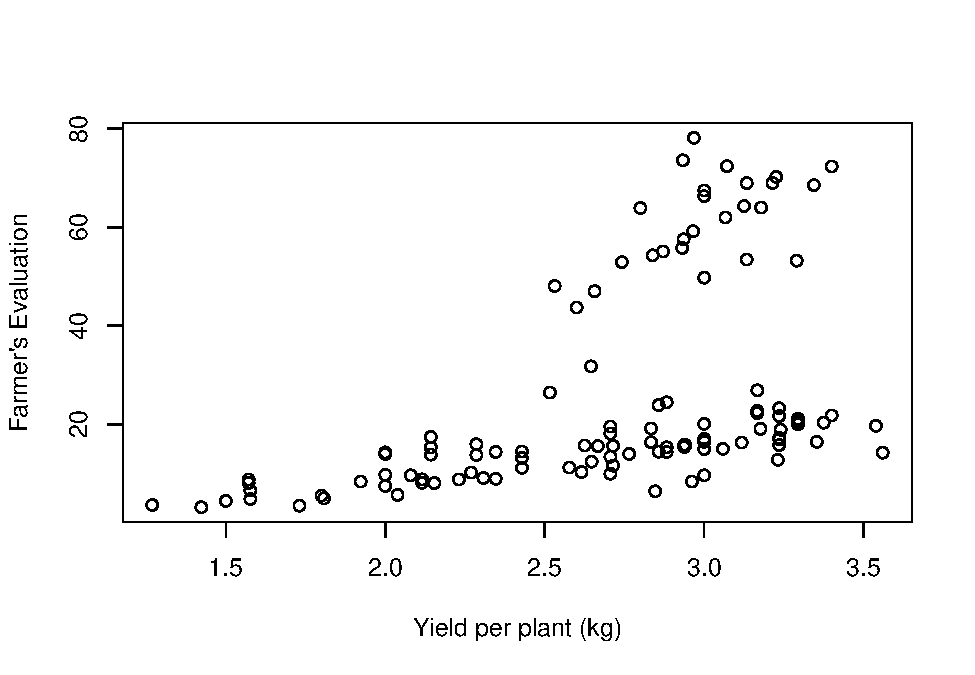
\includegraphics{PPB-Toolkit_files/figure-latex/unnamed-chunk-33-1.pdf}

\hypertarget{another-simple-plot}{%
\section{Another simple plot}\label{another-simple-plot}}

We could, for example plot the harvest data for each location. But first, we will check if the data types are right.

\begin{Shaded}
\begin{Highlighting}[]
\FunctionTok{str}\NormalTok{(mydata)}
\end{Highlighting}
\end{Shaded}

\begin{verbatim}
## 'data.frame':    112 obs. of  9 variables:
##  $ location         : chr  "Molise" "Molise" "Molise" "Molise" ...
##  $ genotype         : chr  "Molise Random" "Sestola Random" "Local Molise" "Modern F1 Hybrid" ...
##  $ repetition       : int  1 1 2 2 1 1 2 2 1 1 ...
##  $ farmers_eval     : num  3.24 2.71 3.35 3.24 3.24 ...
##  $ plant_number     : int  20 20 20 20 20 20 20 20 18 20 ...
##  $ total_harvest    : num  15.79 9.96 16.44 16.93 21.66 ...
##  $ perc_mark_fruits : num  57.5 55.8 76 55.3 81.2 ...
##  $ mean_fruit_weight: num  0.01743 0.00737 0.03554 0.01419 0.06885 ...
##  $ harvest_perplant : num  0.789 0.498 0.822 0.847 1.083 ...
\end{verbatim}

Looks like the location is a character variable, meaning it is just a loose string of text. We rather want it to be a factor, so that all observations with the same location can be grouped in plots.

\begin{Shaded}
\begin{Highlighting}[]
\NormalTok{mydata}\SpecialCharTok{$}\NormalTok{location }\OtherTok{=} \FunctionTok{as.factor}\NormalTok{(mydata}\SpecialCharTok{$}\NormalTok{location)}
\FunctionTok{class}\NormalTok{(mydata}\SpecialCharTok{$}\NormalTok{location)}
\end{Highlighting}
\end{Shaded}

\begin{verbatim}
## [1] "factor"
\end{verbatim}

And now we can do the plot.

\begin{Shaded}
\begin{Highlighting}[]
\FunctionTok{plot}\NormalTok{( }\AttributeTok{x=}\NormalTok{ mydata}\SpecialCharTok{$}\NormalTok{location, }
      \AttributeTok{y=}\NormalTok{mydata}\SpecialCharTok{$}\NormalTok{total\_harvest,}
      \AttributeTok{ylab=} \StringTok{"Total Harvestper plot(kg)"}\NormalTok{,}
      \AttributeTok{xlab=} \StringTok{"Location"}\NormalTok{)}
\end{Highlighting}
\end{Shaded}

\hypertarget{subsetting-your-data.}{%
\section{Subsetting your data.}\label{subsetting-your-data.}}

Suppose you only want to work with a section of your data frame, for example, only the data for one location.

There are many ways to do this, a rather simple one is using the function subset()

\begin{Shaded}
\begin{Highlighting}[]
\NormalTok{soloRotonda }\OtherTok{\textless{}{-}} \FunctionTok{subset}\NormalTok{(mydata, mydata}\SpecialCharTok{$}\NormalTok{location }\SpecialCharTok{==} \StringTok{"Rotonda"}\NormalTok{)}
\FunctionTok{nrow}\NormalTok{(soloRotonda)}
\end{Highlighting}
\end{Shaded}

\begin{verbatim}
## [1] 28
\end{verbatim}

Notice how we created a new subset, only with data from Rotonda. After checking, we see it has only 28 rows, as supposed.

Notice also how we used the ``=='' sign, to express a logical function stating the location had to be equal to ``Rotonda''

In R, the other characters to indicate logical expressions are:\\
* `==' for equal\\
* `!=' for different\\
* `\textless,\textgreater{}' less than, more than\\
* `\textless=' less or equal to\\
* `\textgreater=' more or equal to\\
* `\&' if we want one condition AND another.
* ``\textbar{}'' if we Want one condition OR another.

For example, we can select only the data for Rotonda, in which the evaluation is higher than 3.

\begin{Shaded}
\begin{Highlighting}[]
\NormalTok{soloRotondaSuperiori }\OtherTok{\textless{}{-}} \FunctionTok{subset}\NormalTok{(mydata, }
\NormalTok{                  mydata}\SpecialCharTok{$}\NormalTok{localita}\SpecialCharTok{==} \StringTok{"Rotonda"}
                  \SpecialCharTok{\&} 
\NormalTok{                  mydata}\SpecialCharTok{$}\NormalTok{valutassione\_agricultori }\SpecialCharTok{\textgreater{}=} \DecValTok{3}\NormalTok{)}
\FunctionTok{nrow}\NormalTok{(soloRotondaSuperiori)}
\end{Highlighting}
\end{Shaded}

\begin{verbatim}
## [1] 0
\end{verbatim}

\hypertarget{packages-in-r.}{%
\section{Packages in R.}\label{packages-in-r.}}

Virtually anyone can create and upload a package in R.\\

Some of them are very useful to treat and analyze data. We will see many examples later.\\

Download and installing them is very easy, you have mostly two options./

\begin{enumerate}
\def\labelenumi{\arabic{enumi}.}
\item
  The simplest is to click on Tools \textgreater{} Install Packages \textgreater{} and write the package name.
\item
  You could also write
\end{enumerate}

\begin{Shaded}
\begin{Highlighting}[]
\FunctionTok{install.packages}\NormalTok{(}\StringTok{"yourpackagename"}\NormalTok{)}
\CommentTok{\#Don\textquotesingle{}t try this! It\textquotesingle{}s only an example!}
\end{Highlighting}
\end{Shaded}

Once installed, you have to call it so that it is active on R. This is true for every time you open R.

\begin{Shaded}
\begin{Highlighting}[]
\FunctionTok{library}\NormalTok{(yourpackagename)}
\CommentTok{\#Again, don\textquotesingle{}t try this.}
\end{Highlighting}
\end{Shaded}

For example, we will try to instally DPLYR, which gives us an easy and intuitive grammatic for data manipulation.

\begin{Shaded}
\begin{Highlighting}[]
\FunctionTok{install.packages}\NormalTok{(}\StringTok{"dplyr"}\NormalTok{)}
\FunctionTok{library}\NormalTok{(dplyr)}
\end{Highlighting}
\end{Shaded}

\begin{verbatim}
## 
## Attaching package: 'dplyr'
\end{verbatim}

\begin{verbatim}
## The following objects are masked from 'package:stats':
## 
##     filter, lag
\end{verbatim}

\begin{verbatim}
## The following objects are masked from 'package:base':
## 
##     intersect, setdiff, setequal, union
\end{verbatim}

Some of the most useful functions in Dplyr R are

\begin{Shaded}
\begin{Highlighting}[]
\FunctionTok{filter}\NormalTok{() }\CommentTok{\# To filter rows according to criteria}
\FunctionTok{select}\NormalTok{() }\CommentTok{\# TO select only certain columns}
\FunctionTok{rename}\NormalTok{() }\CommentTok{\# To rename columns. }
\FunctionTok{mutate}\NormalTok{() }\CommentTok{\# TO create a new column from an old one.}
\end{Highlighting}
\end{Shaded}

For example, you can create a new dataframe if you select only location, genotype, repetition and mean fruit weight.

\begin{Shaded}
\begin{Highlighting}[]
\NormalTok{newdataframe }\OtherTok{\textless{}{-}} \FunctionTok{select}\NormalTok{(mydata, location, genotype, repetition, mean\_fruit\_weight)}
\end{Highlighting}
\end{Shaded}

Within this new data frame, I can create a new column, which converts mean fruit weight (now in kg) to grams (g)

\begin{Shaded}
\begin{Highlighting}[]
\NormalTok{newdataframe2 }\OtherTok{\textless{}{-}} \FunctionTok{mutate}\NormalTok{(newdataframe, }\AttributeTok{meanfruitweight\_grams =}\NormalTok{ mean\_fruit\_weight }\SpecialCharTok{*} \DecValTok{1000}\NormalTok{)}
\end{Highlighting}
\end{Shaded}

\hypertarget{the-pipeline-operator}{%
\section{The pipeline \%\textgreater\% operator}\label{the-pipeline-operator}}

With the pipeline operator you can chain more than one operation together, instead of using temporary objects and changing them. It also allows to call my first object (`mydata') only once

\begin{Shaded}
\begin{Highlighting}[]
\NormalTok{newdataframe3 }\OtherTok{\textless{}{-}}\NormalTok{ mydata }\SpecialCharTok{\%\textgreater{}\%}
                 \FunctionTok{select}\NormalTok{(location, genotype, repetition, mean\_fruit\_weight) }\SpecialCharTok{\%\textgreater{}\%}
                 \FunctionTok{mutate}\NormalTok{( }\AttributeTok{meanfruitweight\_grams =}\NormalTok{ mean\_fruit\_weight }\SpecialCharTok{*} \DecValTok{1000}\NormalTok{)}
\end{Highlighting}
\end{Shaded}

\hypertarget{aggregate-data}{%
\section{Aggregate data}\label{aggregate-data}}

Finally, DPLYR helps us us to calculate, for example, the mean perfomance of each genotype per environment, given that there are two repetitions.

For this, you have to use the group\_by() and summarize (). Under group\_by, we put the aggrupating facors. Under summarize, we put the columns we want, in this case, we want the means and the standard deviations.

\begin{Shaded}
\begin{Highlighting}[]
\NormalTok{mydata\_means\_genoxenv }\OtherTok{\textless{}{-}}\NormalTok{ mydata }\SpecialCharTok{\%\textgreater{}\%}
              \FunctionTok{group\_by}\NormalTok{(genotype, location) }\SpecialCharTok{\%\textgreater{}\%}
              \FunctionTok{summarize}\NormalTok{(}\FunctionTok{mean}\NormalTok{(farmers\_eval),}
                          \FunctionTok{sd}\NormalTok{(farmers\_eval),}
                          \FunctionTok{mean}\NormalTok{(harvest\_perplant),}
                         \FunctionTok{sd}\NormalTok{(harvest\_perplant))}
\end{Highlighting}
\end{Shaded}

\hypertarget{save-your-data}{%
\section{Save your data}\label{save-your-data}}

Once you have created and modified and object, you can save it on the same folder in your .csv format.

\begin{Shaded}
\begin{Highlighting}[]
\CommentTok{\#We can save the tomato data with our modifications.}
\FunctionTok{write.csv}\NormalTok{(mydata, }\StringTok{"tomatodata\_modified.csv"}\NormalTok{)}

\CommentTok{\#And we can save the new data frame we created with the means.}
\FunctionTok{write.csv}\NormalTok{(mydata\_means\_genoxenv, }\StringTok{"tomatodata\_means\_genoxenv.csv"}\NormalTok{)}
\end{Highlighting}
\end{Shaded}

\hypertarget{ask-questions}{%
\subsection{Ask questions!}\label{ask-questions}}

It's very hard to know (and remember!) how everything is done.

There will always be things that you want to do, you've never done befora and are out of this very small manual.

Essempi:
1. When wanting to understand a function, you can type ?functionname (and changing ``functionname'' for your actual function.)
2. A great approach is just to google: ``How to \_\_\_\_\_ in R''. This can get you out of many errors.
3. When you receive errors (red letters on the console) try to read them and see what they mean. Another good approach is to copy-paste them in google.

\hypertarget{to-learn-more}{%
\section{To learn more}\label{to-learn-more}}

This are just some sources to learn more about R:

The basic book is the \href{https://rc2e.com/}{R Cookbook}

This is a cool blog to ask questions and learn more: \href{https://stackoverflow.com/}{Stack Overflow}

\hypertarget{methods}{%
\chapter{Methods}\label{methods}}

We describe our methods in this chapter.

\hypertarget{applications}{%
\chapter{Applications}\label{applications}}

Some \emph{significant} applications are demonstrated in this chapter.

\hypertarget{example-one}{%
\section{Example one}\label{example-one}}

\hypertarget{example-two}{%
\section{Example two}\label{example-two}}

\hypertarget{final-words}{%
\chapter{Final Words}\label{final-words}}

We have finished a nice book.

  \bibliography{book.bib,packages.bib}

\end{document}
